\section{Potential}

\begin{figure}
\centering
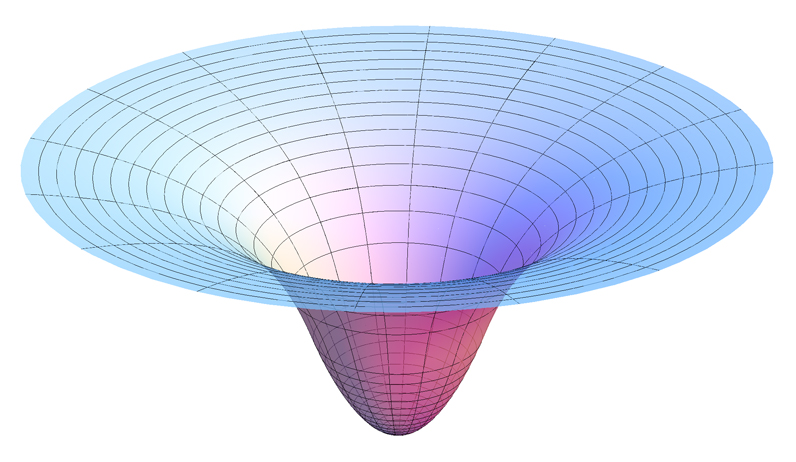
\includegraphics[width=1.0\linewidth]{img/GravityPotential.jpg}
\caption{Gravitational potential around uniform spherical body}
\label{fig:test}
\end{figure}

The gravitational potential $\Phi$ of a unit mass at distance x from some point mass/collection of mass M is defined as work required from the gravitational field F to pull the unit mass into that point from infinitely far away, \\ 

\begin{equation}
\Phi = \frac{W}{m} = 
\frac{1}{m} \int_{\infty}^{x} \! F \, \mathrm{d}x =
\frac{1}{m} \int_{\infty}^{x} \! \frac{GmM}{x^2} \, \mathrm{d}x =
-\frac{GM}{x}
\end{equation}

where W is the work, m is the unit mass and G is the gravitational constant. By convention $\Phi$ is always negative where it is defined, and as x tends to infinity, $\Phi$ approaches zero (see figure 83). 

More generally the gravitational potential of a spherical system can be written as a sum of the potential of this structure from its center out to its radius r, plus the potential term of all surrounding matter in the entire universe: \\ \\

\begin{equation}
\Phi(r) = -4\pi G \Bigg[ \frac{1}{r} \int_0^r \! r'^2 \rho(r') \, \mathrm{d}r' + \int_r^{\infty} \! r' \rho(r') \, \mathrm{d}r' \Bigg]
\end{equation}

%\begin{equation}
%r'
%\end{equation}
%r^{'} and r^{´} and r^' and r^´